\newpage
\section{Continious delay function: Delay of 0}
\begin{figure}[hb]
 %   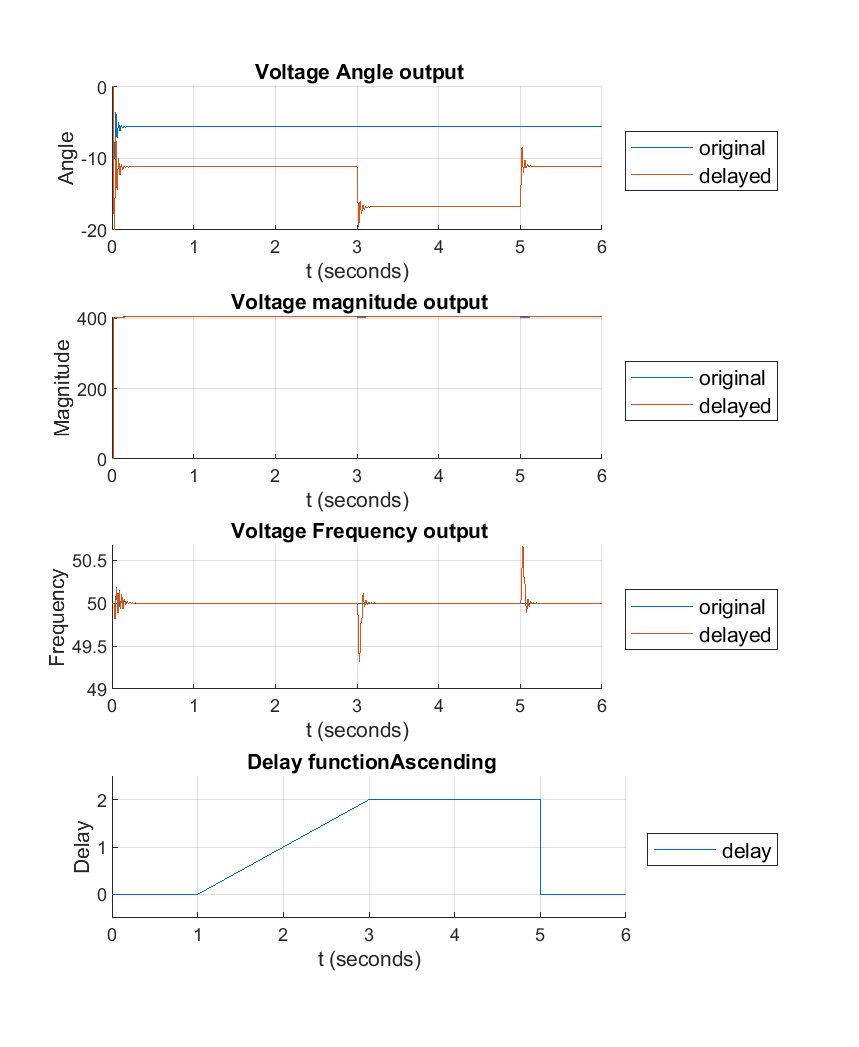
\includegraphics[trim=2 10 14 4, clip]{figures/v_AllFig-DelayOf_2-Ascending.png}    
    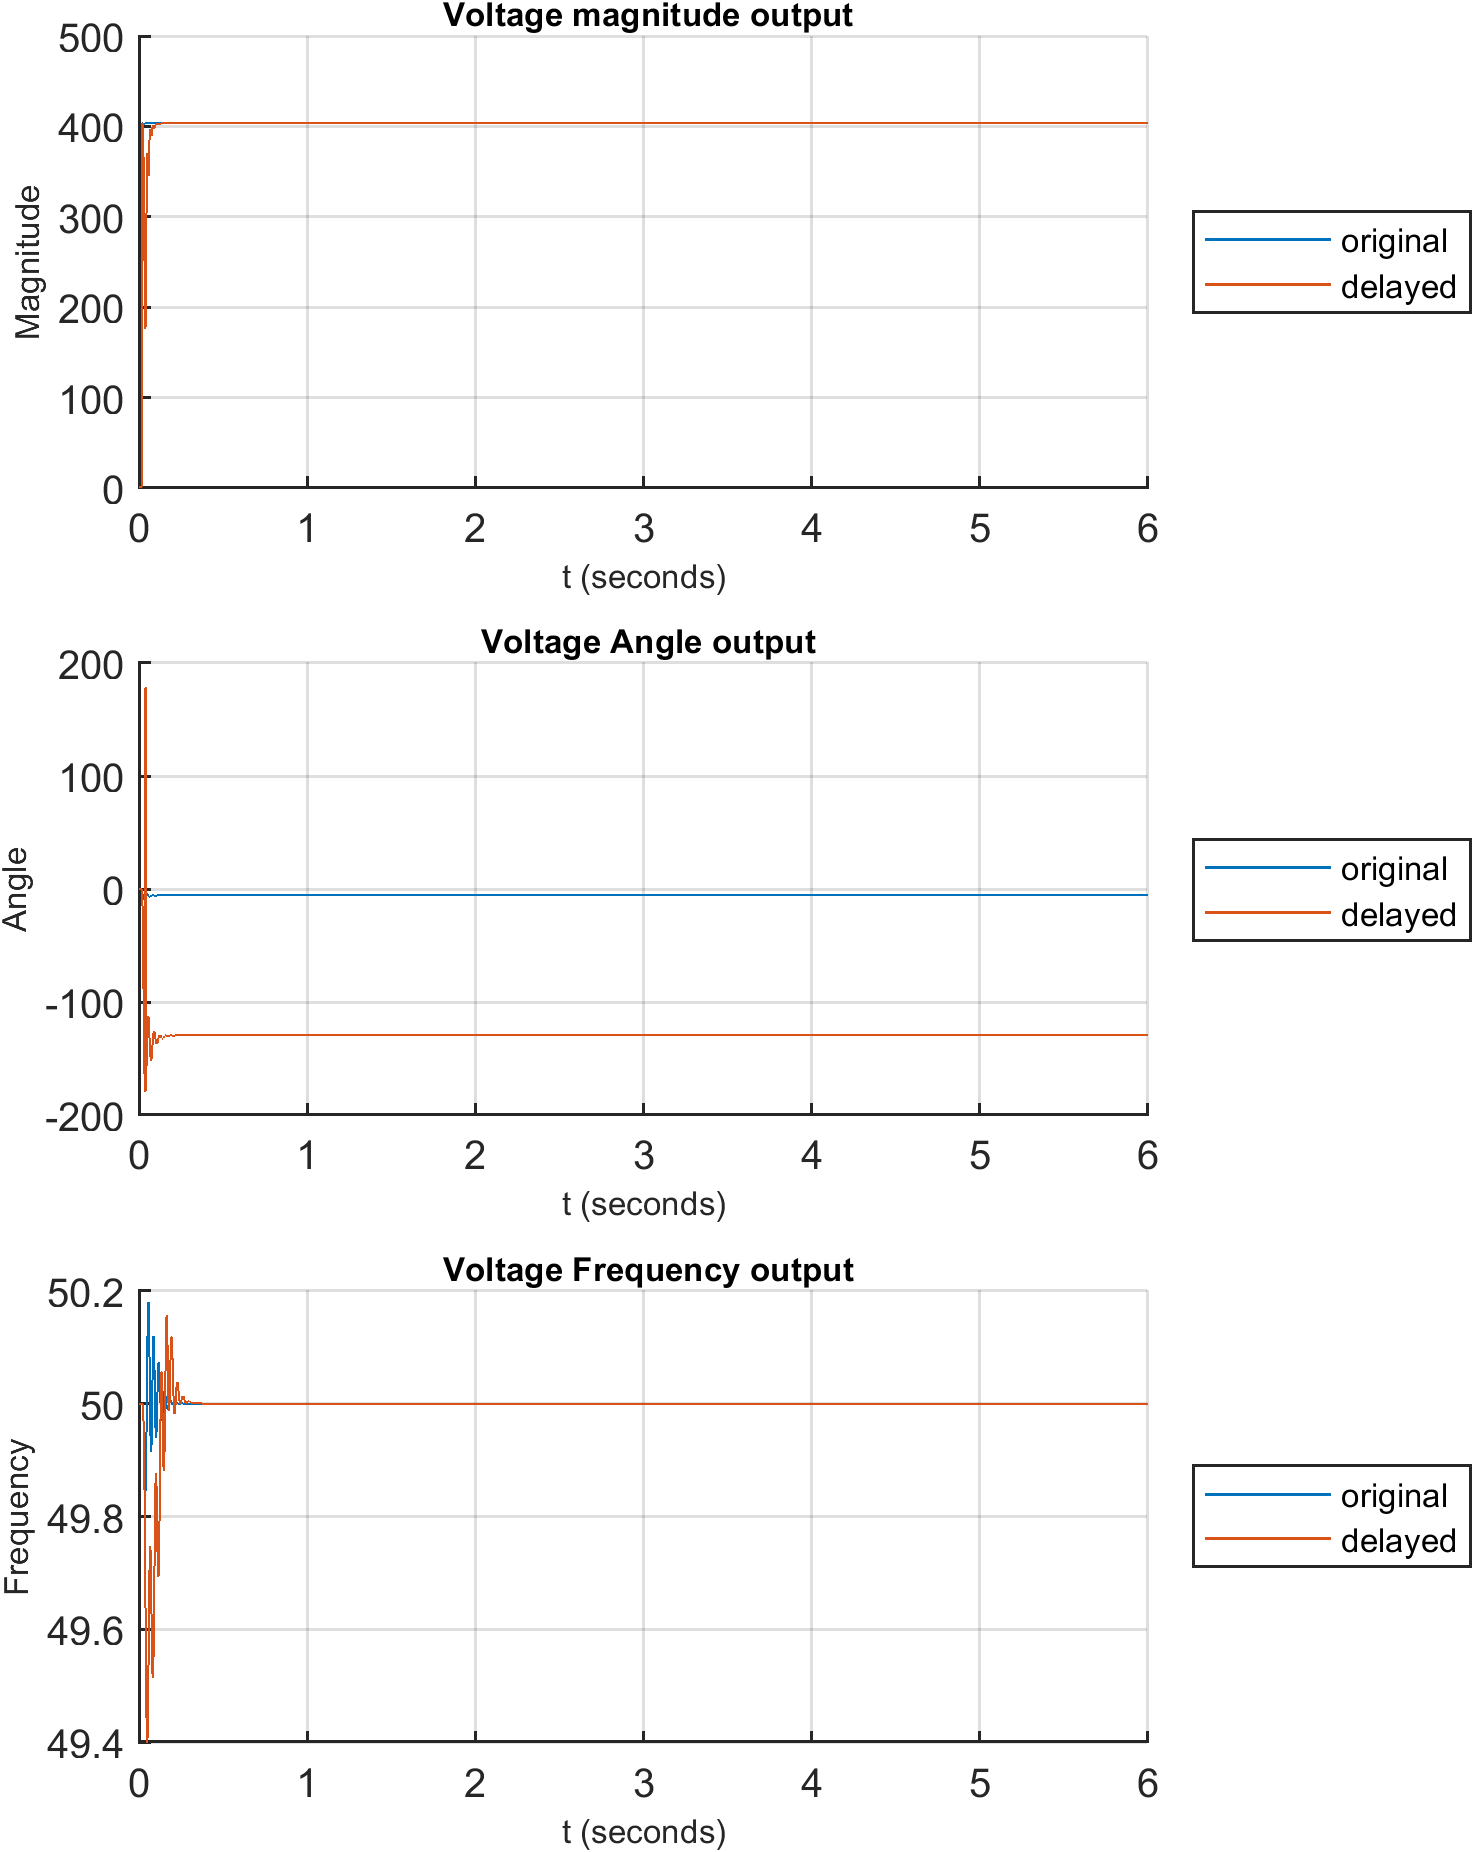
\includegraphics[width=0.95\textwidth]{\locateResults/AllFig.png}    
    \caption{Ascending delay combined output}
    \label{fig:PMUsim-Cont0-allfig}
\end{figure}


     \begin{figure}
        \caption{Component-wise output}
 
    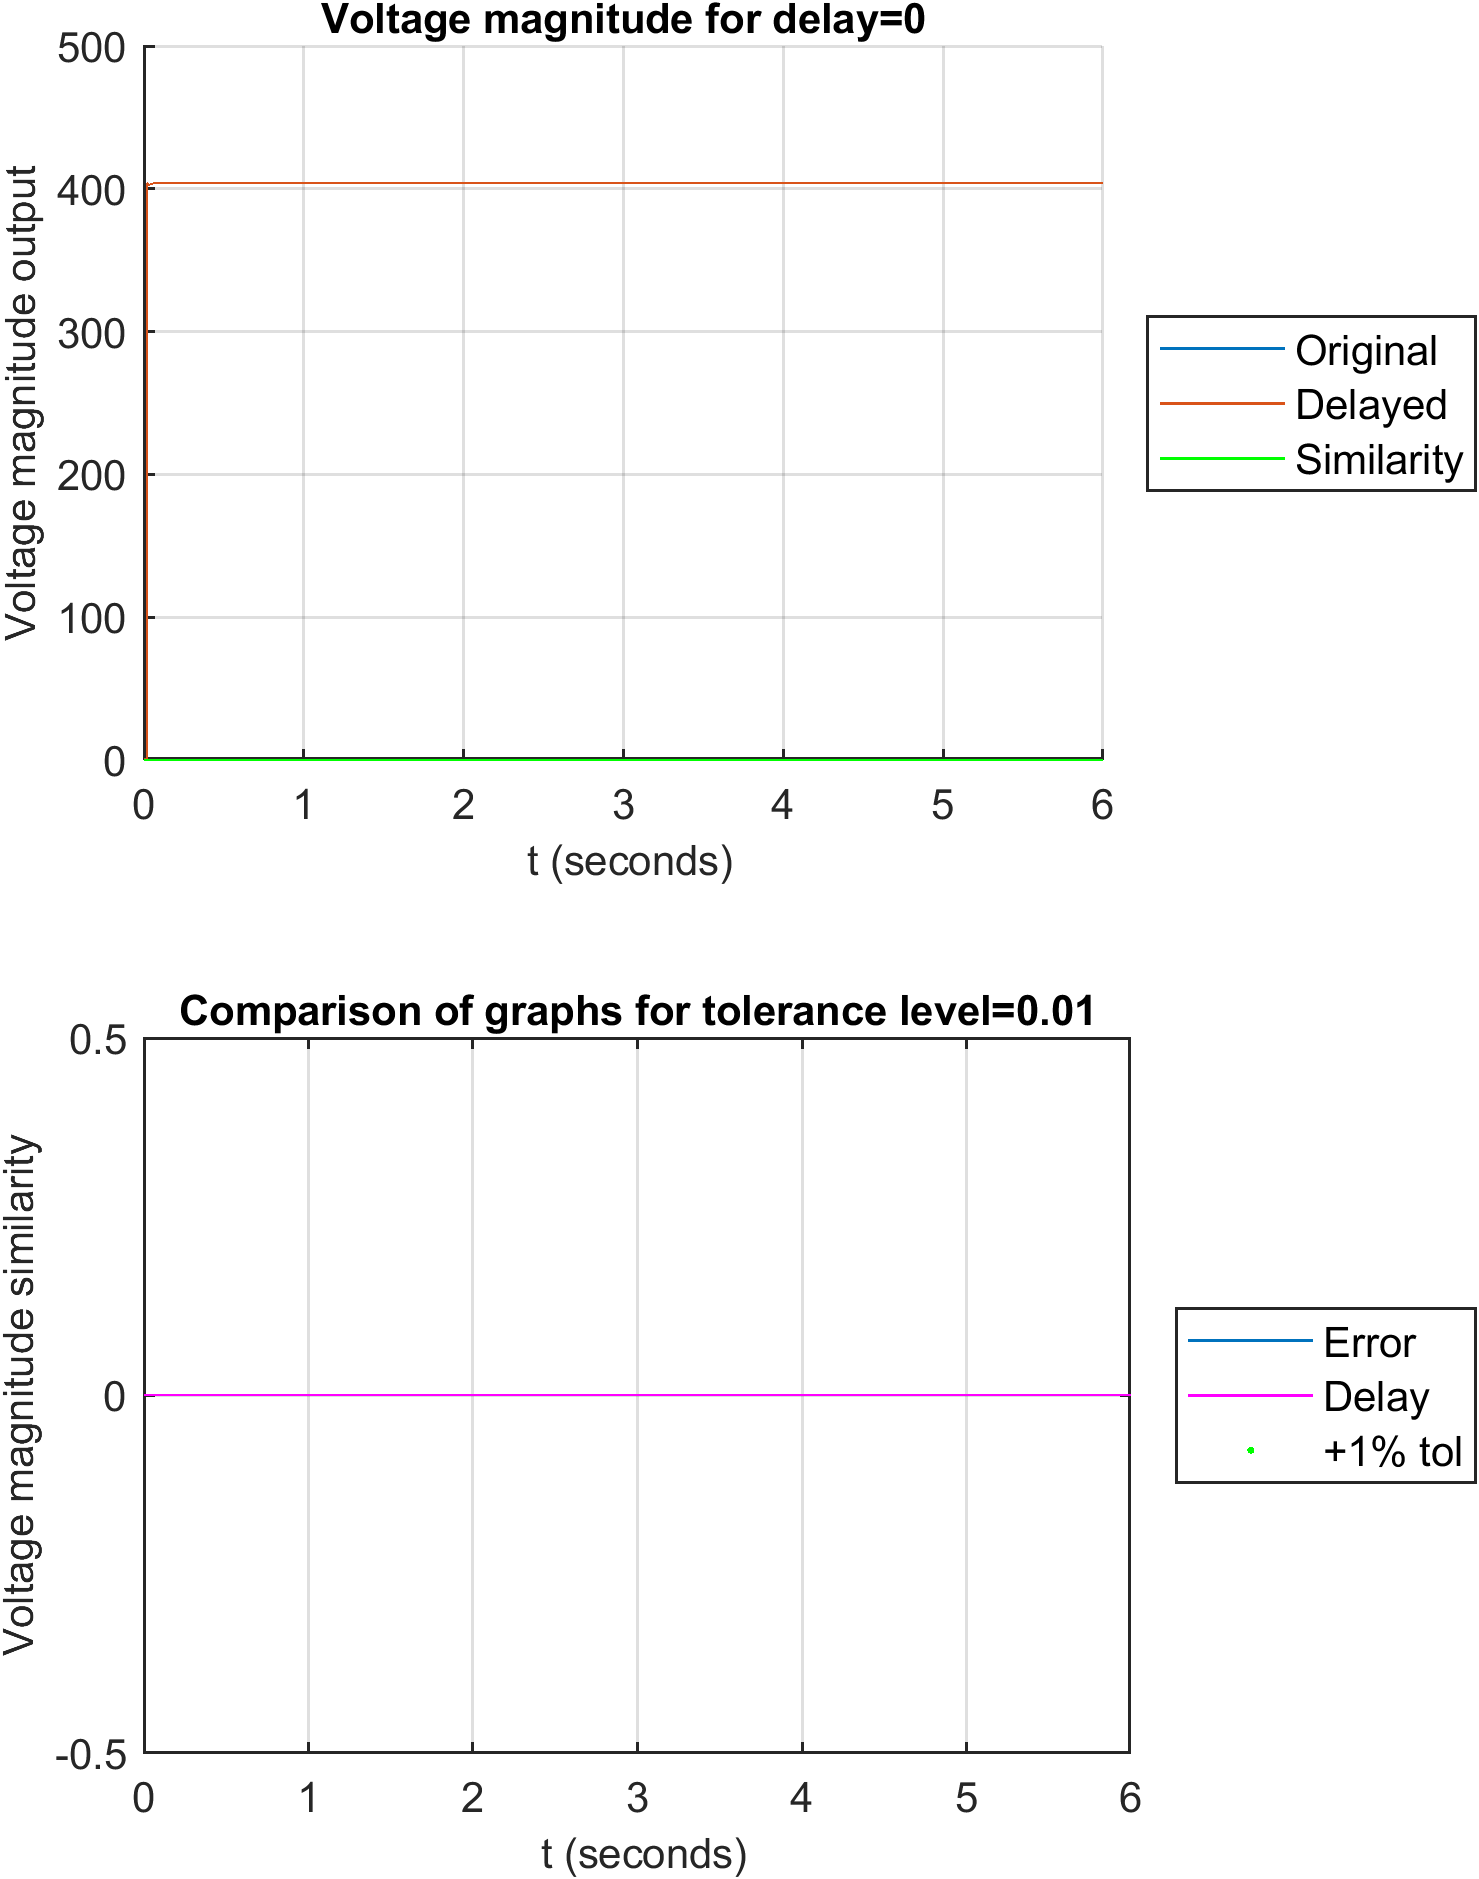
\includegraphics[width=0.95\textwidth]{\locateResults/Magnitude.png}    
         %\caption{magnitude Output}
         \label{fig:PMUsim-Cont0Mag}
   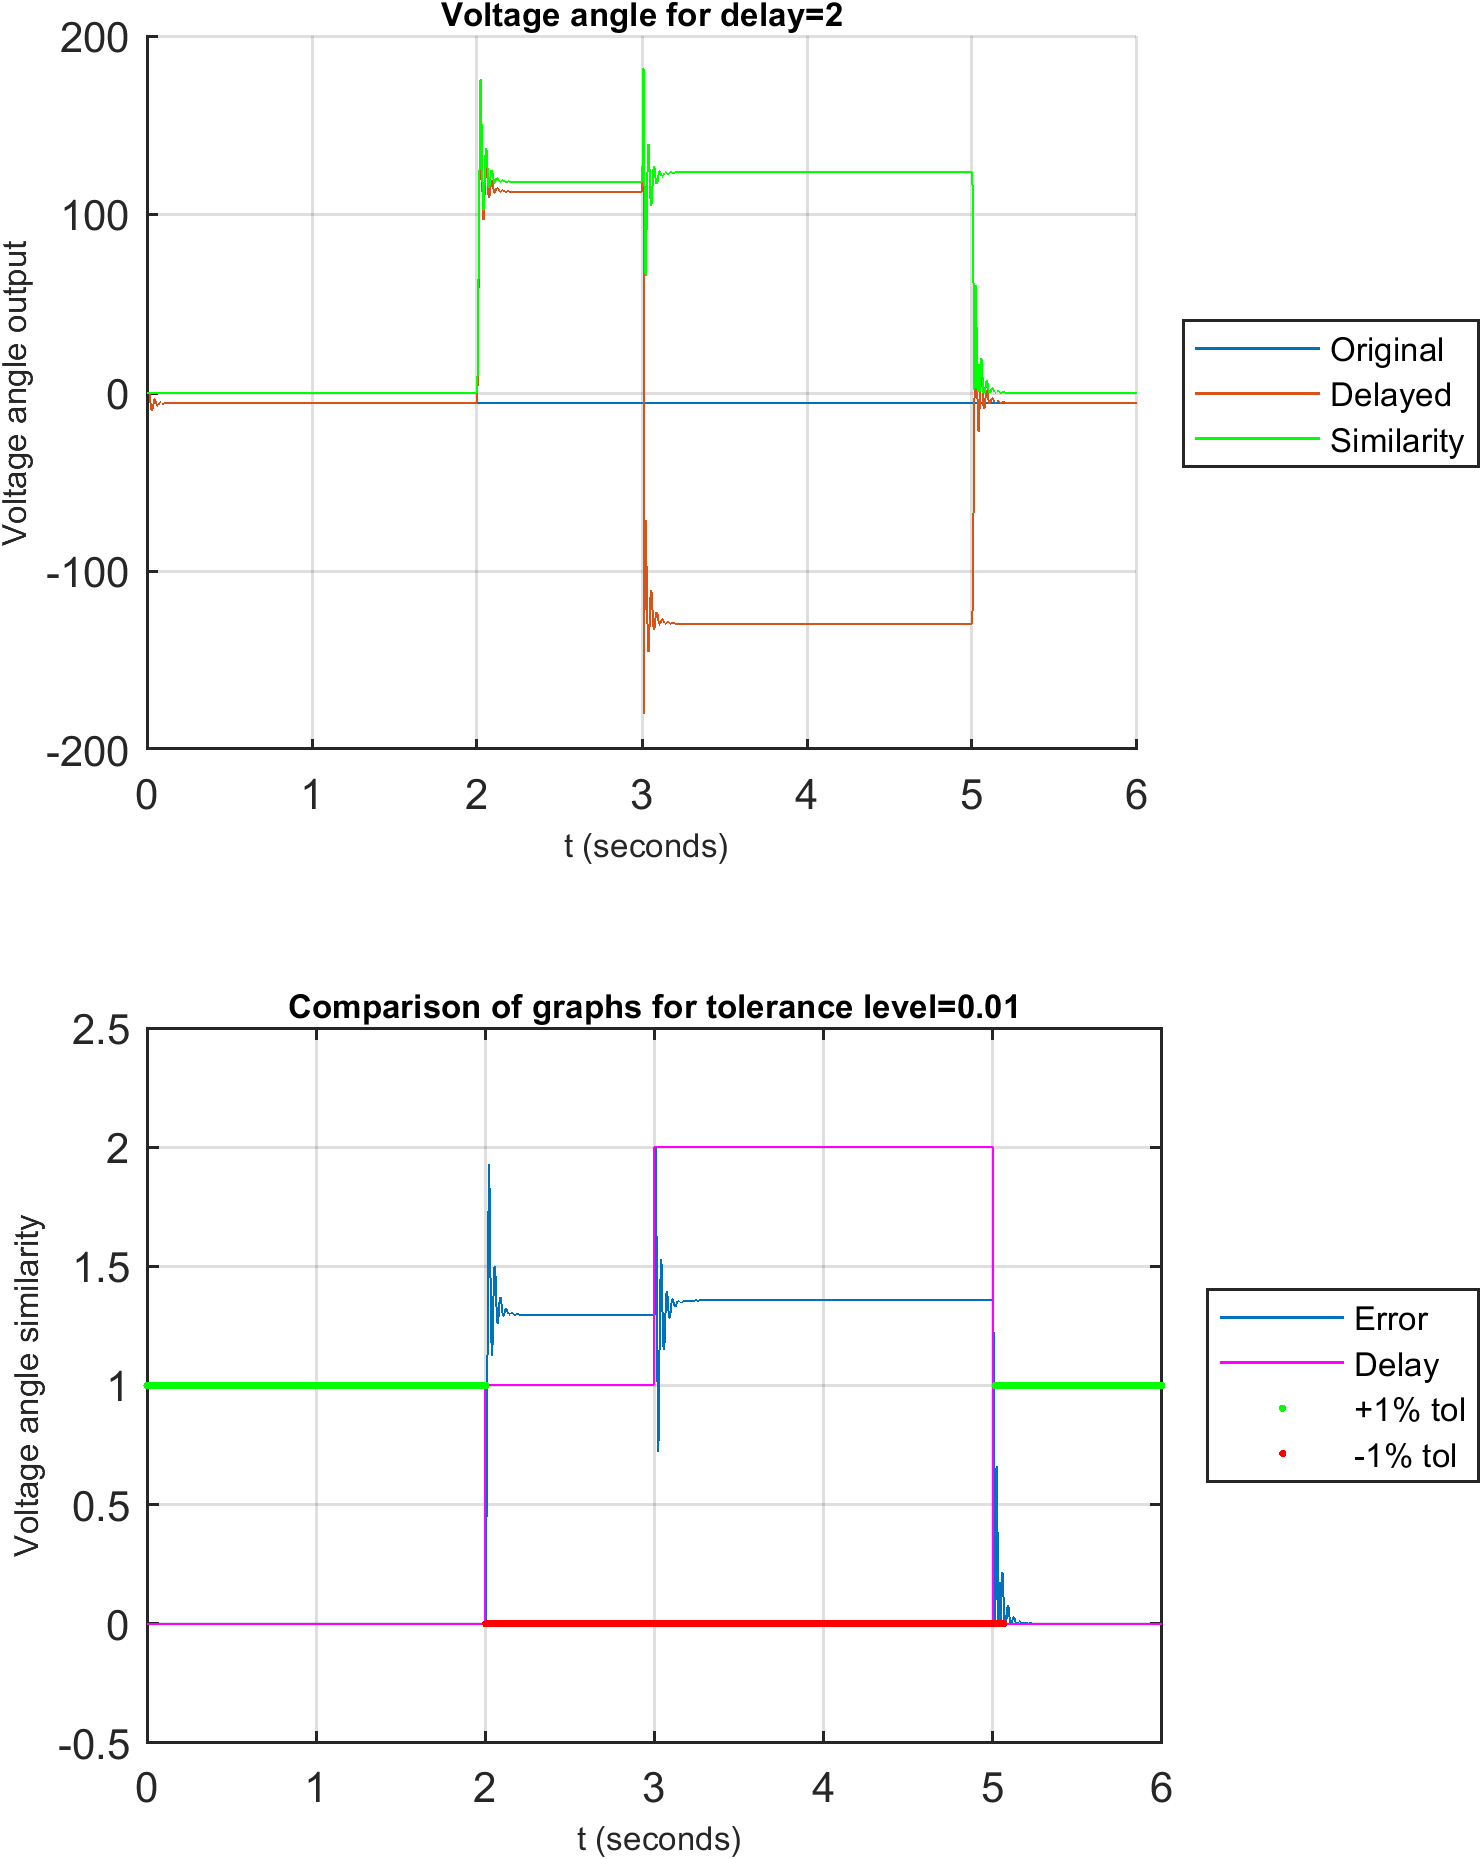
\includegraphics[width=0.95\textwidth]{\locateResults/Angle.png}    
          %\caption{Angle Output}
         \label{fig:PMUsim-Cont0Ang}
   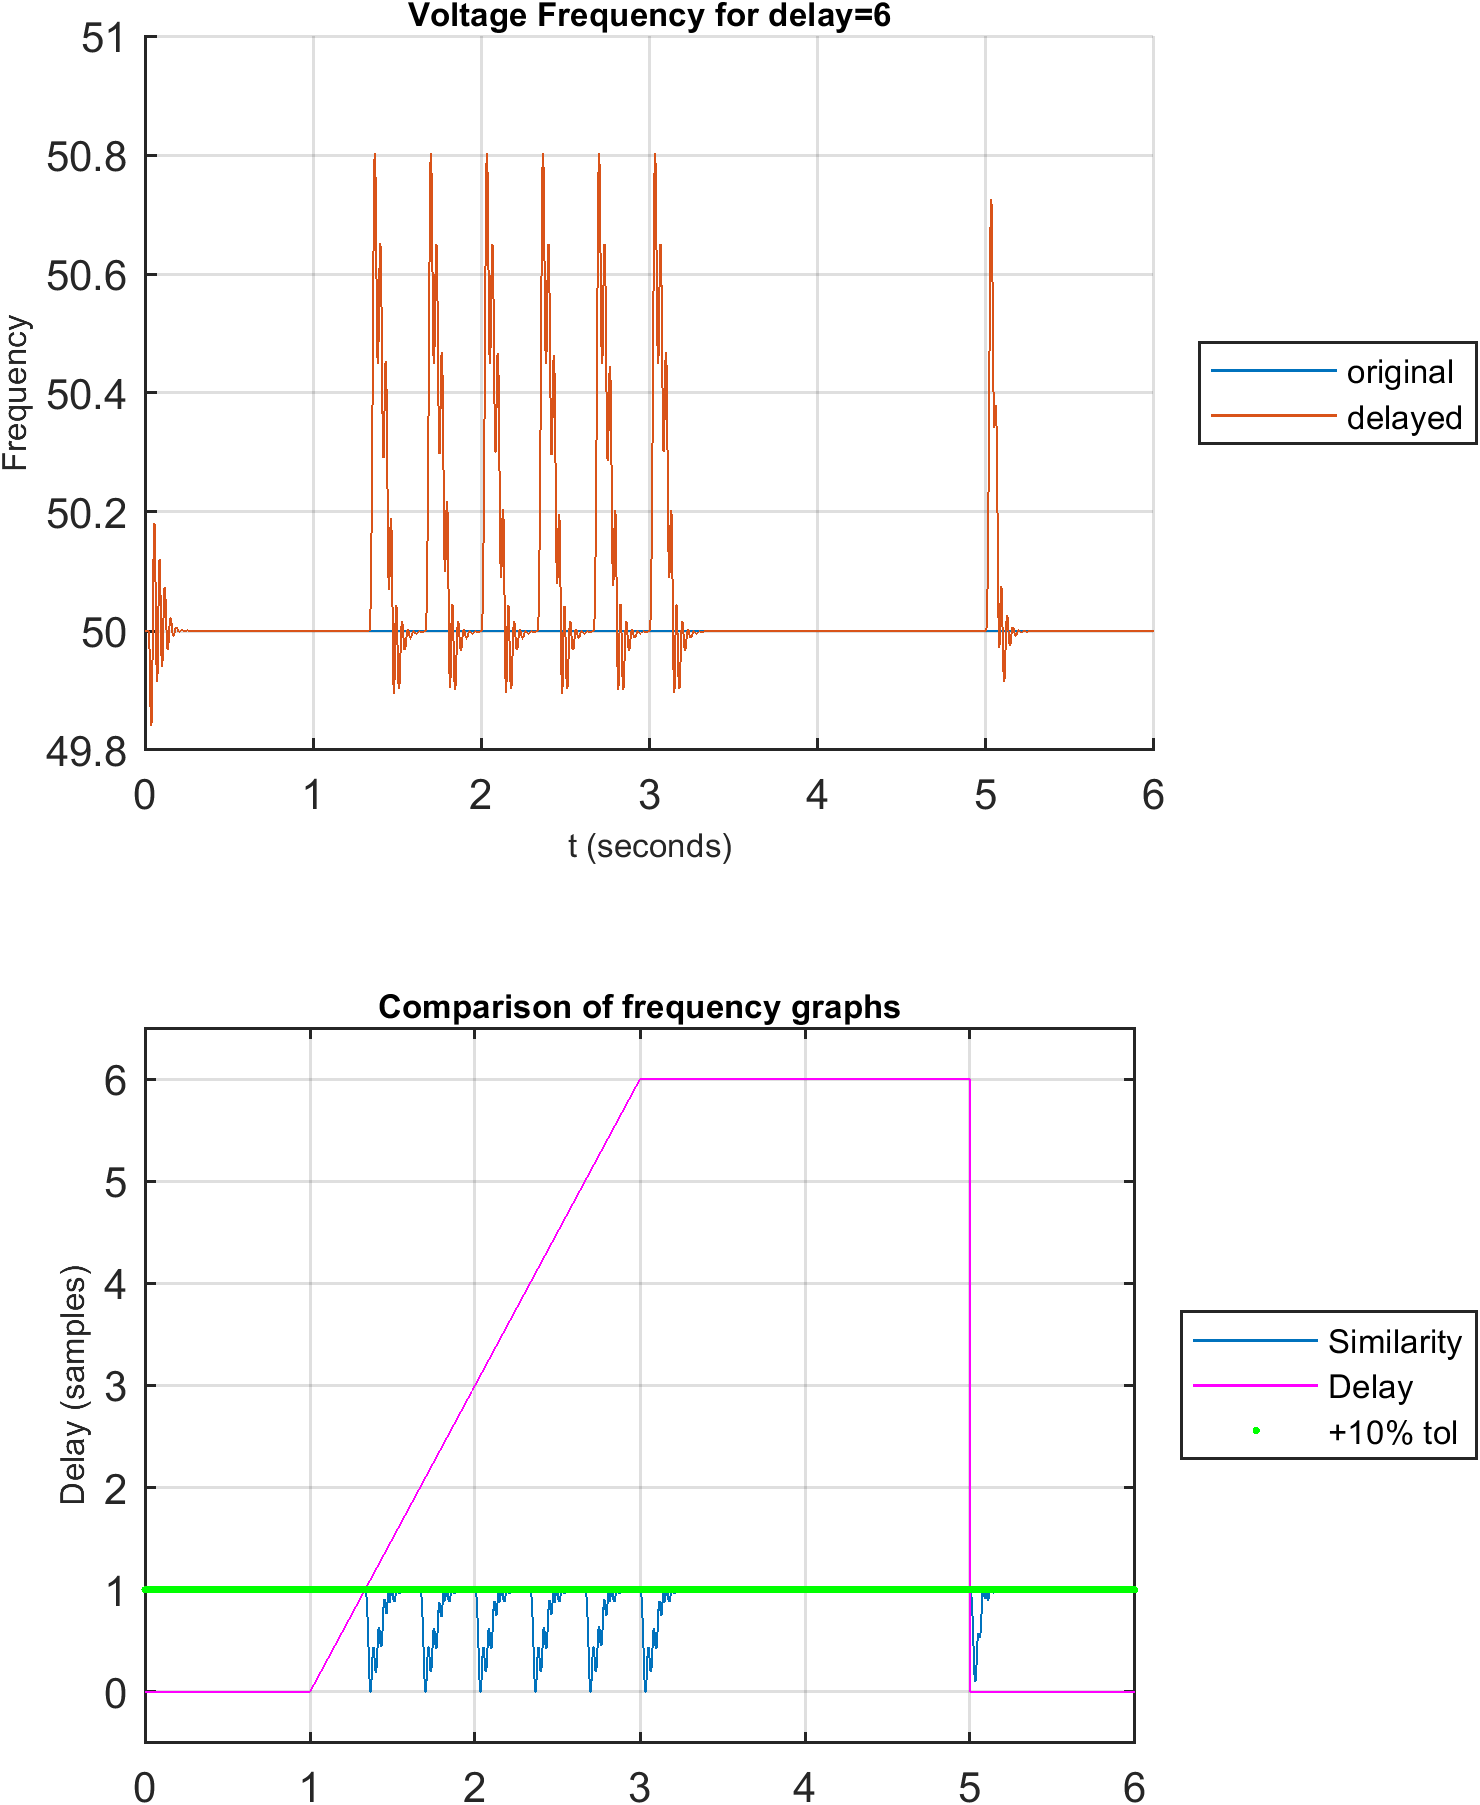
\includegraphics[width=0.95\textwidth]{\locateResults/Frequency.png}    
         %\caption{frequency Output}
         \label{fig:PMUsim-Cont0Freq}
 
\end{figure}


